\section{A continuation-based account of dynamics} \label{sec:cont_based_dyn}

%This section reviews a continuation-based approach introduced in~\cite{deGroote:2006:Towards-a-Montagovian-Account-of-Dynamics} and shows how it handles cross-sentential and donkey anaphora. The approach uses standard tools of mathematical logic, such as simply-typed lambda calculus, and is, therefore, loyal to the Montague's program. 
 
This chapter provides an intuition for the continuation-based framework based on dynamic logic formally defined in Chapter~\ref{}. We begin with discussing the dynamic type of a sentence and its dynamic interpretation in simply-typed lambda calculus.
 
The meaning of a sentence is a function of the context. This can be expressed in lambda calculus by defining the interpretation of a sentence as an abstraction over a variable standing for the context. The notion of context is a complex notion and its formalization is not trivial. Indeed, there exist various proposals of its formalization. \TODO{Put references. Briefly mention these approaches.} 

The framework we propose is not restricted to any specific formalization of a context. In contrast, it provides room for integrating a desired context's representation and the context can be elaborated without affecting the core of the framework. This is achieved by defining the context as a term of a special type $\gamma$ viewed as a parameter. Hence, $\gamma$ can define any complex type.


\begin{definition}[Context, Environment] A \textbf{context} or \textbf{environment} is a term of type $\gamma$ that stores the essential information from what has already been processed in the computation of the meaning of the whole discourse.
\end{definition}

As mentioned above, a sentence is defined as an abstraction over a variable of type $\gamma$. In other words, the sentence awaits for a context. Moreover, the sentence may have a potential to change (update) the context. The update of the context can easily be implemented within the body of the lambda term interpreting the sentence. Furthermore, the updated context has to become available for a \emph{subsequent} sentence. The challenge is to implement this requirement within the interpretation of the current sentence in order to satisfy the compositionality principle. Here is where the notion of continuation is useful. The interpretation of a sentence takes the second argument standing for a continuation. In the body of the sentence, the continuation is provided the updated context as an argument and, therefore, this context becomes available for the future of the computation (and, particularly, for the subsequent sentence). We consider the continuation fed with the context to be an additional conjunct in the body of the term interpreting the sentence.


 We shall clarify the type of continuation. As discussed above, it serves for providing current (possibly updated) context to the future of the computation. Therefore, it is a function that has an argument of type $\gamma$. Since continuation applied to the context is an additional conjunct in the logical interpretation of the sentence, the continuation should return a proposition when given a context. Consequently, the continuation is defined as a term of type $(\gamma \rightarrow o)$.


\begin{definition}[Continuation] A \textbf{continuation} is a term of type $(\gamma \rightarrow o)$ that denotes what is still to be processed in the computation of the meaning of the whole discourse. 
\end{definition}

 Thereupon, we define the meaning of a sentence as a function of two arguments, a context $e$ of type $\gamma$ and a continuation $\phi$ of type $(\gamma \rightarrow o)$, that returns a proposition:
\begin{align}
\I{s} = \underbrace{\gamma}_{\begin{smallmatrix}
\text{type of}\\
\text{context}
\end{smallmatrix}} \rightarrow \underbrace{(\gamma \rightarrow o)}_{\begin{smallmatrix}
\text{type of}\\
\text{continuation}
\end{smallmatrix}} \rightarrow \underbrace{o}_{
\begin{smallmatrix}
\text{type of}\\
\text{proposition}
\end{smallmatrix}} \notag
\end{align}

Consequently, we define $(\gamma \rightarrow (\gamma \rightarrow o) \rightarrow o)$ to be the type of a dynamic proposition:
\begin{definition}[Type of a dynamic proposition] Every dynamic proposition is a term of type $(\gamma \rightarrow (\gamma \rightarrow o) \rightarrow o)$.
\end{definition}


Example~\ref{ex:2006-jlm} shows the dynamic meaning~\eqref{eq:ex:lovejm} of the simple sentence~\eqref{sent:JlovesM-2006}. Note the presence of the conjunct $\phi e^*$ in~\eqref{eq:ex:lovejm} that conveys that an updated context is passed as an argument to the continuation of a proposition, and is, therefore, accessible in the rest of the computation. As mentioned above, this kind of conjunct is a subterm of every proposition in the dynamic approach.
 \begin{example} \label{ex:2006-jlm} The meaning of the sentence~\eqref{sent:JlovesM-2006} is the lambda-term~\eqref{eq:ex:lovejm}:\footnote{We interpret objects as variables, i.e. as terms of type $\iota$.}
\enumsentence{ \txt{John loves Mary.} \label{sent:JlovesM-2006}}
\begin{align}
\underbrace{\lambda \overbrace{\underbrace{e^{\gamma}}_{\text{context}} \underbrace{\phi^{\gamma \rightarrow o}}_{\text{continuation}}.  \overbrace{\overbrace{ \overbrace{\textbf{love}^{\iota \rightarrow \iota \rightarrow o}  \ \textbf{j}^{\iota}}^{\iota \rightarrow o} \ \textbf{m}^{\iota}}^{o} \land \overbrace{\phi e^*}^{o}}^{o}}^{\gamma \rightarrow (\gamma \rightarrow o) \rightarrow o} }_{\text{dynamic proposition}} \label{eq:ex:lovejm}
%\underbrace{\underbrace{a+b}_\textrm{brace1} + c + d}_\textrm{brace2}
\end{align}
\indent where  $e^*$ is the context obtained by updating $e$.
\end{example}

 Context $e^*$ is just an abbreviation in~\eqref{eq:ex:lovejm}. To have the complete representation of the context, we should first decide what the parameter $\gamma$ is standing for. We will consider here a simple definition of $\gamma$ as a list of individuals:
\begin{align} \label{def:gammaislistofiota}
\gamma \defeq \texttt{ list of } [ \ \iota \ ]  
\end{align}
 
 
 This choice of the simple representation of the context is motivated  by our preference to focus on the mechanism of our compositional framework and avoid being distracted from this goal with the discussion what the ideal interpretation of the context should be. Indeed, the definition~\eqref{def:gammaislistofiota} of $\gamma$ is already sufficient for illustrating the basic idea of the approach on handling cross-sentential and donkey anaphora.
 

The context defined in~\eqref{def:gammaislistofiota}  stores interpretations of objects that previously occurred in the discourse. When a new object is interpreted as an individual $x$, the current context $e$ is updated with $x$, resulting in $(x::e)$, where $::$ is a list constructor of type $(\iota \rightarrow \gamma \rightarrow \gamma)$:

\begin{notation}[List constructor] The list constructor $::$ is a function that takes an individual and a context and returns an (updated) context:
\begin{align} 
 \I{::}  =  \iota \rightarrow \gamma \rightarrow \gamma
\end{align}
\end{notation}

\begin{remark}
Operation $::$ is right associative. For example, $(x::y::e)$ is equivalent to $(x::(y::e))$.
\end{remark}

Having defined the list constructor, we can substitute $e^*$ with the more precise $(\textbf{m} :: \textbf{j} ::{e})$ in Example~\ref{ex:2006-jlm}. Consequently, Sentence~\eqref{sent:JlovesM-2006} is more accuratly interpreted as follows:
\begin{align}
\lambda e \phi. \textbf{love}  \ \textbf{j} \ \textbf{m} \land \phi (\textbf{m} :: \textbf{j} ::{e}) \label{eq:ex:lovejm-2}
\end{align}

Term~\eqref{eq:ex:lovejm-2} has to be computed compositionally from lexical meanings $\I{John}$, $\I{Mary}$ and $\I{loves}$. More precisely, it has to be the result of normalizing  $\I{loves} \I{Mary} \I{John}$, as can be seen from the syntactic tree in Figure~\ref{fig:JohnLovesMary}.
\begin{figure}[h!]
 \centering
    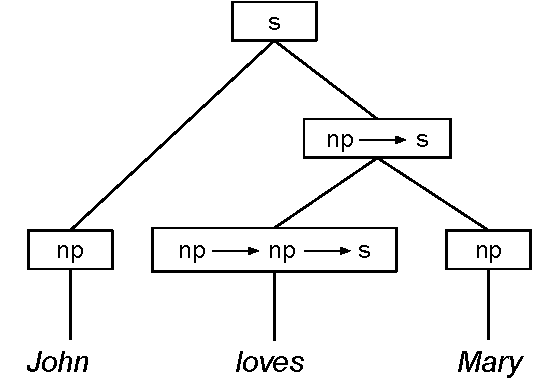
\includegraphics[width=0.4\textwidth]{images/JohnLovesMary.pdf}
\caption{Syntactic parse tree of sentence \txt{John loves Mary}.} \label{fig:JohnLovesMary}
\end{figure}

A noun phrase in Montague semantics is a term taking a property as an argument and returning a proposition.  As motivated above, there should be two additional arguments (one standing for context and one standing for continuation) for a term to return a proposition in our dynamic framework. Therefore, everywhere where a term of type $o$ occurs in Montague's interpretation, there has to be a term of type $(\gamma \rightarrow (\gamma \rightarrow o) \rightarrow o)$ in the dynamic framework. This can be easily seen comparing~\eqref{eq:np:M:1} and~\eqref{eq:np:dG:1}, where $\Omega$ is an abbreviation for $(\gamma \rightarrow (\gamma \rightarrow o) \rightarrow o)$. Thus, a noun phrase is interpreted as a function of three arguments (a property, a context and a continuation) that returns a proposition, as can be more easily seen in~\eqref{eq:np:dG:2}, where no abbreviation is used:
\begin{subequations}
\begin{align}
\I{np} =_{Montague} \ & \underbrace{(\iota \rightarrow   o)}_{
\begin{smallmatrix}
\text{static}\\
\text{property}
\end{smallmatrix}} \rightarrow \underbrace{o}_{\begin{smallmatrix} 
\text{static}\\
\text{proposition}
\end{smallmatrix}} \label{eq:np:M:1} \\
\I{np} =_{de~Groote} \ & \underbrace{(\iota \rightarrow  \Omega )}_{\begin{smallmatrix}
\text{dynamic}\\
\text{property}
\end{smallmatrix}} \rightarrow \underbrace{\Omega}_{
\begin{smallmatrix}
\text{dynamic}\\
\text{proposition}
\end{smallmatrix}} \label{eq:np:dG:1} \\
\I{np} =_{de~Groote} \ & \underbrace{(\iota \rightarrow \gamma \rightarrow (\gamma \rightarrow o) \rightarrow o)}_{
\begin{smallmatrix}
\text{dynamic}\\
\text{property}
\end{smallmatrix}} \rightarrow \underbrace{\underbrace{\gamma}_{\text{context}} \rightarrow \underbrace{(\gamma \rightarrow o)}_{\text{continuation}} \rightarrow \underbrace{o}_{\text{proposition}}}_{\begin{smallmatrix}
\text{dynamic}\\
\text{proposition}
\end{smallmatrix}} \label{eq:np:dG:2}
\end{align}
\label{eq:np:MdG}
\end{subequations}

The interpretation of \txt{Mary}, for example, is as follows: 
\begin{align}
\I{Mary} =  \overbrace{\lambda \underbrace{{\P2}^{\iota \rightarrow \gamma \rightarrow (\gamma \rightarrow o) \rightarrow o}}_{\begin{smallmatrix}
\text{dynamic}\\
\text{property}
\end{smallmatrix}}. \underbrace{\lambda \underbrace{{e}^{\gamma}}_{\text{context}} \underbrace{{\phi}^{\gamma \rightarrow o}}_{\text{continuation}}. \overbrace{\overbrace{\overbrace{\P2 {\textbf{m}}^{\iota}}^{\gamma \rightarrow (\gamma \rightarrow o) \rightarrow o} e}^{(\gamma \rightarrow o) \rightarrow o} \ \ (\overbrace{\lambda e'^{\gamma}. \overbrace{\phi ( \overbrace{\upii{\textbf{m}}{e'}}^{\gamma})}^{o}}^{\gamma \rightarrow o})}^{o}}_{
\begin{smallmatrix}
\text{dynamic}\\
\text{proposition}
\end{smallmatrix}}}^{(\iota \rightarrow \gamma \rightarrow (\gamma \rightarrow o) \rightarrow o) \rightarrow \gamma \rightarrow (\gamma \rightarrow o) \rightarrow o}\label{eq:dG:Mary}
\end{align}

The interpretation of \txt{John} is analogous:
\begin{align}
\I{John} = \lambda \P2. \lambda e \phi. \P2 \textbf{j} e (\lambda e' .\phi (\textbf{j}::{e'})) \label{eq:dG:John}
\end{align}

A transitive verb is interpreted in Montague semantics as a term taking two type-raised individuals and returning a proposition.  Since in the dynamic framework there has to be an abstraction over a context and a continuation to get a proposition,  everywhere where a term of type $o$ occurs in Montague's interpretation, there has to be a term of type $(\gamma \rightarrow (\gamma \rightarrow o) \rightarrow o)$ in de Groote's interpretation. This can be seen comparing types in~\eqref{eq:tv:MdG}:
\begin{subequations}
\begin{align}
\I{tv} =_{Montague} \ & (\underbrace{(\iota \rightarrow   o)}_{\text{property}} \rightarrow \underbrace{o}_{\text{proposition}}) \rightarrow (\underbrace{(\iota \rightarrow   o)}_{\text{property}} \rightarrow \underbrace{o}_{\text{proposition}})  \rightarrow \underbrace{o}_{\text{proposition}} \\
\I{tv} =_{de~Groote} \ &  (\underbrace{(\iota \rightarrow   \Omega)}_{\text{property}} \rightarrow \underbrace{\Omega}_{\text{proposition}}) \rightarrow (\underbrace{(\iota \rightarrow   \Omega)}_{\text{property}} \rightarrow \underbrace{\Omega}_{\text{proposition}})  \rightarrow \underbrace{\Omega}_{\text{proposition}} 
\end{align} \label{eq:tv:MdG}
\end{subequations}

Then the interpretation of \txt{loves} is as follows:
\begin{align}
\I{loves} = \overbrace{\lambda \Y2^{(\iota \rightarrow \Omega) \rightarrow \Omega} \X2^{(\iota \rightarrow \Omega) \rightarrow \Omega}.  \overbrace{\X2 ( \overbrace{\lambda \x1.  \overbrace{\Y2 ( \overbrace{\lambda \y1. (  \overbrace{\lambda {e'}^{\gamma} \phi^{\gamma \rightarrow o}. \overbrace{\overbrace{\overbrace{{\textbf{love}}^{\iota \rightarrow \iota \rightarrow o} {\x1}^{\iota}}^{\iota \rightarrow o} {\y1}^{\iota}}^{o} \land \overbrace{\phi e'}^{o}}^{o} )}^{\Omega}}^{\iota \rightarrow \Omega} )}^{\Omega}}^{\iota \rightarrow \Omega} )}^{\Omega} }^{((\iota \rightarrow \Omega) \rightarrow \Omega) \rightarrow ((\iota \rightarrow \Omega) \rightarrow \Omega) \rightarrow \Omega} \label{eq:dG:love}
\end{align}



\begin{example}[$\S_1$, \txt{John loves Mary}] Now, given lexical interpretations~\eqref{eq:dG:love},~\eqref{eq:dG:Mary} and~\eqref{eq:dG:John} of \txt{loves}, \txt{Mary} and \txt{John} respectively, the meaning~\eqref{eq:ex:lovejm-2} (\eqref{eq:2006:JohnLovesMary} below) of Sentence~\eqref{sent:JlovesM-2006}  can be computed compositionally:
\begin{align}
\S_1 = \ & \I{loves} \I{Mary} \I{John}  \notag \\
= \ & (\lambda \Y2 \X2. \X2( \lambda \x1. \Y2 (\lambda \y1. ( \lambda e' \phi. \textbf{love} \x1 \y1 \land \phi e' ))) )  \I{Mary} \I{John}  \notag \\
\bconv \ & (\lambda  \X2. \X2( \lambda \x1. \I{Mary}  (\lambda \y1. ( \lambda e' \phi. \textbf{love} \x1 \y1 \land \phi e' ))) )  \I{John}  \notag \\
\bconv \ &    \I{John}( \lambda \x1. \I{Mary}  (\lambda \y1. ( \lambda e' \phi. \textbf{love} \x1 \y1 \land \phi e' )))   \notag \\
= \ &    \I{John}( \lambda \x1. (\lambda \P2. \lambda e \phi. \P2 \textbf{m} e (\lambda e. \phi (\upii{\textbf{m}}{e'})))  (\lambda \y1. ( \lambda e' \phi. \textbf{love} \x1 \y1 \land \phi e' )))   \notag \\
\bconv \ &    \I{John}( \lambda \x1.  \lambda e \phi. (\lambda \y1. ( \lambda e' \phi. \textbf{love} \x1 \y1 \land \phi e' )) \textbf{m} e (\lambda e'. \phi (\upii{\textbf{m}}{e'})))   \notag \\
\bconv \ &    \I{John}( \lambda \x1.  \lambda e \phi. ( \lambda e' \phi. \textbf{love} \x1 \textbf{m} \land \phi e' ) e (\lambda e' . \phi (\upii{\textbf{m}}{e'})))   \notag \\
\bred \ &  \I{John}( \lambda \x1.  \lambda e \phi.  \textbf{love} \x1 \textbf{m} \land  (\lambda e' .\phi (\upii{\textbf{m}}{e'}) e))   \notag \\
\bconv \ &  \I{John}( \lambda \x1.  \lambda e \phi.  \textbf{love} \x1 \textbf{m} \land  \phi (\upii{\textbf{m}}{e} ))   \notag \\
= \ &    ( \lambda \P2. \lambda e \phi. \P2 \textbf{j} e (\lambda e' .\phi (\upii{\textbf{j}}{e'})))( \lambda \x1.  \lambda e \phi.  \textbf{love} \x1 \textbf{m} \land  \phi (\upii{\textbf{m}}{e} ))   \notag \\
\bconv \ &    \lambda e \phi. ( \lambda \x1.  \lambda e \phi.  \textbf{love} \x1 \textbf{m} \land  \phi (\upii{\textbf{m}}{e} ))   \textbf{j} e (\lambda e' . \phi (\upii{\textbf{j}}{e'})) \notag \\
\bred \ &    \lambda e \phi.  \textbf{love}  \textbf{j} \textbf{m} \land   (\lambda e' .\phi (\upii{\textbf{j}}{e'})) (\upii{\textbf{m}}{e} )  \notag \\
\bconv \ &    \lambda e \phi.  \textbf{love}  \textbf{j} \textbf{m} \land   \phi (\upii{\textbf{j}}{\upii{\textbf{m}}{e} })   \label{eq:2006:JohnLovesMary} 
\end{align}
\end{example}

To cope with anaphora, the context has to be accessed. This can be accomplished by defining a special function $\selK$ of type $(\gamma \rightarrow \iota)$ that takes a context and returns an individual. Assuming that $\selK$ implements an anaphora resolution algorithm and  works as an oracle always retrieving the correct antecedent makes it possible to interpret pronouns as shown, for example, for \txt{he} below:
\begin{align}
\I{he} =  \overbrace{\lambda \P2^{^\iota \rightarrow \gamma \rightarrow (\gamma \rightarrow o) \rightarrow o}. \lambda e^{\gamma} \phi^{\gamma \rightarrow o}. \overbrace{\overbrace{\overbrace{\P2 ( \overbrace{\selK_{he} e}^{\iota} )}^{\gamma \rightarrow (\gamma \rightarrow o) \rightarrow o} e}^{ (\gamma \rightarrow o) \rightarrow o} \ \phi }^{o}}^{(\iota \rightarrow \gamma \rightarrow (\gamma \rightarrow o) \rightarrow o) \rightarrow \gamma \rightarrow (\gamma \rightarrow o) \rightarrow o}  \label{eq:he:2006}
%\I{he} = \lambda \P2. \lambda e \phi. \P2 (\selK_{he}e)e\phi
\end{align}

\begin{example}[$\S_2$, \txt{He smiles at her}] \label{ex:2006:HeSmilesAtHer} The meaning of the sentence~\eqref{HeSmilesAtHer-2006} computed in accordance with the parse-tree in Figure~\ref{fig:ptS3-2006}  is as follows:
\enumsentence{\txt{He smiles at her.} \label{HeSmilesAtHer-2006}}
\begin{align}
\S_2 = \ & \I{smiles\_at} \I{her} \I{he} \notag \\
 = \ & (\lambda \Y2 \X2. \X2( \lambda \x1. \Y2 (\lambda \y1. ( \lambda e' \phi. \textbf{smile} \x1 \y1 \land \phi e' ))) )  \I{her} \I{he} \notag \\
\bconv \ & (\lambda  \X2. \X2( \lambda \x1.  \I{her}  (\lambda \y1. ( \lambda e' \phi. \textbf{smile} \x1 \y1 \land \phi e' ))) ) \I{he} \notag \\
\bconv \ &   \I{he} ( \lambda \x1.  \I{her}  (\lambda \y1. ( \lambda e' \phi. \textbf{smile} \x1 \y1 \land \phi e' ))) \notag  \\
= \ &   \I{he} ( \lambda \x1.  (\lambda \P2. \lambda e \phi. \P2 (\selK_{her}e)e\phi)  (\lambda \y1. ( \lambda e' \phi. \textbf{smile} \x1 \y1 \land \phi e' ))) \notag \\
 \bconv \ &   \I{he} ( \lambda \x1.  (\lambda e \phi.  (\lambda \y1. ( \lambda e' \phi. \textbf{smile} \x1 \y1 \land \phi e' )) (\selK_{her}e)e\phi) ) \notag \\
  \bconv \ &   \I{he} ( \lambda \x1.  (\lambda e \phi.   ( \lambda e' \phi. \textbf{smile} \x1  (\selK_{her}e) \land \phi e' ) e\phi) ) \notag \\
 \bred \ &   \I{he} ( \lambda \x1.  (\lambda e \phi.  \textbf{smile} \x1  (\selK_{her}e) \land \phi e) ) \notag \\
  = \ &  (\lambda \P2. \lambda e \phi. \P2 (\selK_{he}e)e\phi) ( \lambda \x1.  (\lambda e \phi.  \textbf{smile} \x1  (\selK_{her}e) \land \phi e) ) \notag \\
\bconv \ & \lambda e \phi. ( \lambda \x1.  (\lambda e \phi.  \textbf{smile} \x1  (\selK_{her}e) \land \phi e) )  (\selK_{he}e)e\phi \notag \\
\bconv \ & \lambda e \phi.   (\lambda e \phi.  \textbf{smile}  (\selK_{he}e)  (\selK_{her}e) \land \phi e) e\phi \notag \\
\bred \ & \lambda e \phi.   \textbf{smile}  (\selK_{he}e)  (\selK_{her}e) \land \phi e \label{eq:2006:HeSmilesAtHer}
\end{align}
\end{example}

\begin{figure}[h]
 \centering
    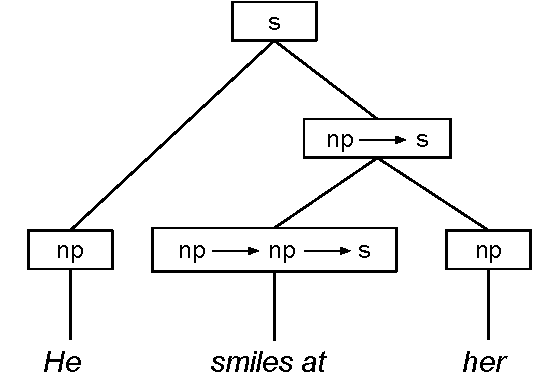
\includegraphics[width=0.4\textwidth]{images/HeSmilesatHer.pdf}
\caption{Syntactic parse tree of sentence \txt{He smiles at her}.} \label{fig:ptS3-2006}
\end{figure}

As Example~\ref{ex:2006:HeSmilesAtHer} shows, Sentence~\eqref{HeSmilesAtHer-2006} is meaningful in the sense that it has an interpretation~\eqref{eq:2006:HeSmilesAtHer}. However, the function $\selK$ can return individuals for \txt{he} and \txt{her} only when the sentence is evaluated over some context containing the corresponding antecedents. This happens when the sentence is uttered in a discourse. The pronominal anaphora can then be resolved during the update of the meaning of the discourse with the meaning of the sentence. 

Discourses can, like sentences, be interpreted as terms of type $(\gamma \rightarrow (\gamma \rightarrow o) \rightarrow o)$.  The update of a discourse interpreted as $\D$ with a sentence interpreted as $\S$ results in interpretation $\updt \ \D \ \S$ of a new discourse. This interpretation is defined by the following equation:
\begin{align}
\updt \ \D \ \S \defeq \overbrace{\lambda e^{\gamma} \phi^{\gamma \rightarrow o}. \overbrace{ \overbrace{\D^{\gamma \rightarrow (\gamma \rightarrow o) \rightarrow o}  e}^{(\gamma \rightarrow o) \rightarrow o} (\overbrace{\lambda e'^{\gamma}. \overbrace{\overbrace{\S^{\gamma \rightarrow (\gamma \rightarrow o) \rightarrow o}  e'}^{ (\gamma \rightarrow o) \rightarrow o} \phi}^{o}}^{\gamma \rightarrow o})}^{o}}^{\gamma \rightarrow (\gamma \rightarrow o) \rightarrow o} \label{eq:updtDS:2006}
\end{align}

\TODO{Take an empty discourse. Feed it with Sentence 1. Feed the result with Sentence 2.}

\begin{example}[$\updt \ \D \ \S$]
Now interpretations~\eqref{eq:2006:JohnLovesMary} and~\eqref{eq:2006:HeSmilesAtHer} can be composed through equation~\eqref{eq:updtDS:2006}, regarding~\eqref{sent:JlovesM-2006} as the discourse updated with the sentence~\eqref{HeSmilesAtHer-2006}. This leads to the interpretation of the piece of discourse~\eqref{sen:JLMHeSH:2006}:
\enumsentence{\txt{John loves Mary. He smiles at her.} \label{sen:JLMHeSH:2006}}
\begin{align}
& \lambda e \phi. (\overbrace{\lambda e \phi.  \textbf{love}  \textbf{j} \textbf{m} \land   \phi (\upii{\textbf{j}}{\upii{\textbf{m}}{e} }) }^{\D}  ) e (\lambda e'. (\overbrace{\lambda e \phi.   \textbf{smile}  (\selK_{he}e)  (\selK_{her}e) \land \phi e}^{\S}) e' \phi ) \notag \\
\bred \ & \lambda e \phi. (\lambda e \phi.  \textbf{love}  \textbf{j} \textbf{m} \land   \phi (\upii{\textbf{j}}{\upii{\textbf{m}}{e} }) ) e (\lambda e'.  \textbf{smile}  (\selK_{he}e')  (\selK_{her}e') \land \phi e' ) \notag \\
\bred \ & \lambda e \phi.\textbf{love}  \textbf{j} \textbf{m} \land    (\lambda e'.  \textbf{smile}  (\selK_{he}e')  (\selK_{her}e') \land \phi e' )  (\upii{\textbf{j}}{\upii{\textbf{m}}{e} }) \notag \\
\bconv \ & \lambda e \phi.\textbf{love}  \textbf{j} \textbf{m} \land    \textbf{smile}  (\selK_{he}(\upii{\textbf{j}}{\upii{\textbf{m}}{e} }))  (\selK_{her}(\upii{\textbf{j}}{\upii{\textbf{m}}{e} })) \land \phi  (\upii{\textbf{j}}{\upii{\textbf{m}}{e} }) \label{int:JLMHeSH:2006}
\end{align}
\end{example}

%Interpretation~\eqref{int:JLMHeSH:2006} of the discourse consisting of the utterance of~\eqref{sen:JLMHeSH:2006} is computed in a compositional manner. 
Note that in the resulting interpretation~\eqref{int:JLMHeSH:2006}, the context of the interpretation of the first sentence is passed to $\selK$ operators of the interpretation of the second sentence. Assuming that an anaphora resolution mechanism is implemented in $\selK$, the following semantic representation of~\eqref{sen:JLMHeSH:2006} is obtained: 
\begin{align}
\lambda e \phi.\textbf{love} \  \textbf{j} \ \textbf{m} \land    \textbf{smile}  \ \textbf{j} \ \textbf{m} \land \phi  (\upii{\textbf{j}}{\upii{\textbf{m}}{e} }) \label{int:JLMHeSH:2006-2}
\end{align}
The context $(\upii{\textbf{j}}{\upii{\textbf{m}}{e} })$ in~\eqref{int:JLMHeSH:2006} (and hence in~\eqref{int:JLMHeSH:2006-2}) being the argument of the continuation $\phi$ is accessible for future computation. This means that the individuals $\textbf{j}$ and $\textbf{m}$ can serve as ancestors for anaphoric pronouns in the following sentences. 
